
Divide y vencer\'as es una t\'ecnica algor\'itmica que consiste en resolver un problema divi\'endolo en problemas m\'as pequeños y combinando las soluciones. 
El proceso de divisi\'on contin\'ua hasta que los subproblemas llegan a ser lo suficientemente sencillos como para una resoluci\'on directa.

El hecho de que el tamaño de los subproblemas sea estrictamente menor que el tamaño original del problema nos garantiza la convergencia hacia los casos elementales.
El coste computacional se determina resolviendo relaciones de recurrencia.

Una forma de dirigir las cartas siguiendo este m\'etodo (creada por Donald Knuth, autor de The Art of Computer Programming) es separarlas en bolsas diferentes en funci\'on de su \'area geogr\'afica y cada una a su vez se ordena en lotes para subregiones más pequeñas.
 
Un ejemplo anterior a Cristo donde se usa \"divide y vencerás\" \ con un \'unico subproblema es el algoritmo de Euclides para computar el máximo com\'un divisor de dos n\'umeros.
 
\begin{figure}[htb] 
\centering
	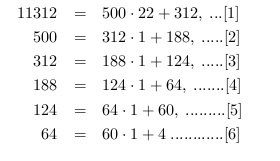
\includegraphics[width=0.40\textwidth]{./Imagenes/euclides.jpg}
	\caption{Euclides} 
	\label{fig:euclides} 
\end{figure}